\documentclass{standalone}

\usepackage{pgfplots}
\usepackage{tikz}

\pgfplotsset{compat=newest}
\usepgfplotslibrary{groupplots}

\begin{document}
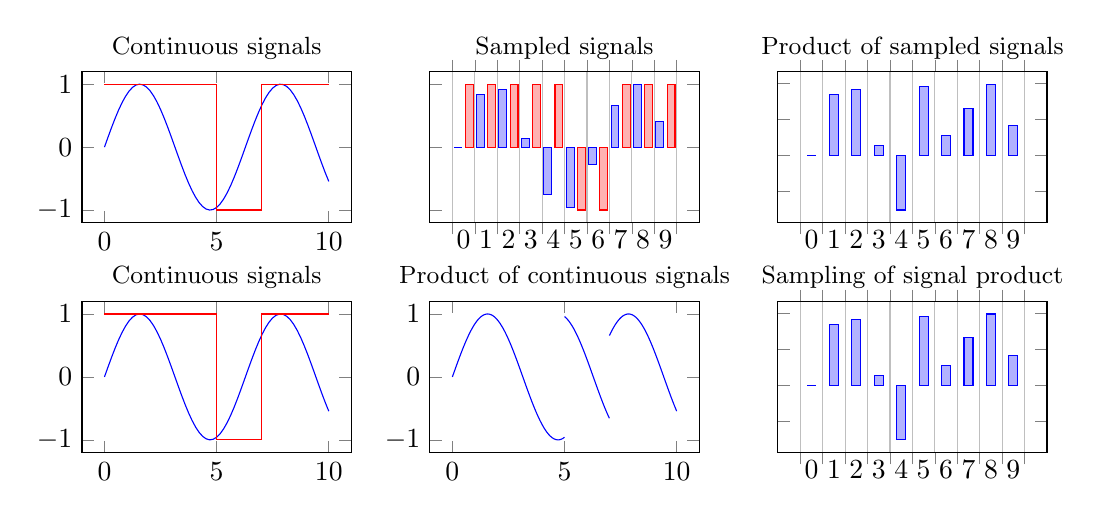
\begin{tikzpicture}
  \begin{groupplot}[group style={group size=3 by 2}, domain=0:10, height=3.5cm, width=5cm, no markers, title style={yshift=-5pt,font=\small}]
    \nextgroupplot[samples=65, title={Continuous signals}]
    \addplot {sin(deg(x))}; 
    \addplot coordinates {(0,1) (5,1) (5,-1) (7,-1) (7,1) (10,1)};
    % \legend{$x$,$y$}
    \nextgroupplot[ybar interval=0.7, samples=11, yticklabels={,,},, title={Sampled signals},xticklabel style = {yshift=5pt}]
    \addplot {sin(deg(x))};
    \addplot coordinates {(0,1) (1,1) (2,1) (3,1) (4,1) (5,-1) (6,-1) (7,1) (8,1) (9,1) (10,1)};   
    % \legend{$x$,$y$}
    \nextgroupplot[ybar interval=0.4, samples=11, yticklabels={,,}, y filter/.code={\pgfmathparse{#1 * sin(deg(x))}\pgfmathresult}, , title={Product of sampled signals},xticklabel style = {yshift=5pt}]
    \addplot coordinates {(0,1) (1,1) (2,1) (3,1) (4,1) (5,-1) (6,-1) (7,1) (8,1) (9,1) (10,1)};
    % \legend{$x+y$}
    %%%%%%%%%%%%%%%%%%%%%%%%%%%%%%%%%%%%%%%%%%%%%%%%%
    \nextgroupplot[samples=65, title={Continuous signals}]
    \addplot {sin(deg(x))}; 
    \addplot coordinates {(0,1) (5,1) (5,-1) (7,-1) (7,1) (10,1)};
    % \legend{$x$,$y$}
    \nextgroupplot[samples=65, title={Product of continuous signals}]
    \addplot[blue,domain=0:5] {sin(deg(x))}; 
    \addplot[blue,domain=5:7] {-sin(deg(x))}; 
    \addplot[blue,domain=7:10] {sin(deg(x))}; 
    % \legend{$x+y$}
    \nextgroupplot[ybar interval=0.4, samples=11, yticklabels={,,}, y filter/.code={\pgfmathparse{#1 * sin(deg(x))}\pgfmathresult}, , title={Sampling of signal product},xticklabel style = {yshift=5pt}]
    \addplot coordinates {(0,1) (1,1) (2,1) (3,1) (4,1) (5,-1) (6,-1) (7,1) (8,1) (9,1) (10,1)};
    % \legend{$x+y$}
  \end{groupplot}
\end{tikzpicture}
\end{document}

%%% Local Variables:
%%% mode: latex
%%% TeX-master: t
%%% End:
